\documentclass[conference]{IEEEtran}
\IEEEoverridecommandlockouts

\usepackage{cite}
\usepackage{amsmath,amssymb,amsfonts}
\usepackage{algorithmic}
\usepackage{graphicx}
\usepackage{textcomp}
\usepackage{xcolor}
\usepackage{grffile}
\usepackage{float}

\def\BibTeX{{\rm B\kern-.05em{\sc i\kern-.025em b}\kern-.08em
T\kern-.1667em\lower.7ex\hbox{E}\kern-.125emX}}

\begin{document}

\title{A Low-Power Hybrid Flip-Flop using\\ Sleepy Stack Inverter Pairs:\\
A Replication and Extension Study\\
{\footnotesize \textsuperscript{*}Complex Engineering Problem of Linear Integrated Circuit Designing}
}

\author{
\IEEEauthorblockN{1\textsuperscript{st} Waseem Akram}
\IEEEauthorblockA{\textit{Department of ECE} \\
\textit{Air University}\\
Islamabad, Pakistan \\
200771@students.au.edu.pk}
\and
\IEEEauthorblockN{2\textsuperscript{nd} Ali Abdullah}
\IEEEauthorblockA{\textit{Department of ECE} \\
\textit{Air University}\\
Islamabad, Pakistan \\
200695@students.au.edu.pk}
\and
\IEEEauthorblockN{3\textsuperscript{rd} Abdul Mohsin}
\IEEEauthorblockA{\textit{Department of ECE} \\
\textit{Air University}\\
Islamabad, Pakistan \\
200773@students.au.edu.pk}
}

\maketitle

\begin{abstract}
This study presents a low-power hybrid flip-flop design that integrates sleepy stack inverters into the static stage of a conventional dual dynamic node pulsed hybrid flip-flop (DDFF) to enhance power efficiency during the evaluation and pre-charge phases. Notably effective in reducing leakage power in advanced technology nodes ($<$90nm), the sleepy stack inverters were compared against a conventional DDFF baseline in Cadence Virtuoso 90nm. The proposed design achieved a 20\% reduction in total power consumption and an 89\% reduction in leakage power at the output node. A derived T flip-flop based on this design also outperformed the conventional DDFF in minimizing leakage power, total power usage, and power-delay product, especially at higher speeds. The design is a promising candidate for high-performance applications requiring substantial power efficiency gains in advanced semiconductor technologies.\footnote{This work was completed as a Complex Engineering Problem (CEP) course project. It replicates Park \& Mooney (2006) and Absel et al.~(2013), and extends them by integrating sleepy stack inverters into the DDFF static stage.}
\end{abstract}

\begin{IEEEkeywords}
Flip Flop, Sleepy Stack Inverter, Leakage Power, Low Power, Leakage Reduction
\end{IEEEkeywords}

\section{Introduction}

Flip-flops serve as indispensable components within synchronous sequential digital circuits, offering crucial functionalities in data storage and signal synchronization. These essential elements are commonly designed in two primary styles: dynamic logic style, known for its high speed and compact area utilization, and static logic style, favored for its low-power attributes. However, the pursuit of an ideal flip-flop has led to the conception of hybrid designs, amalgamating the advantages of both dynamic and static architectures.

In this context, our focus narrows on a hybrid flip-flop configuration, leveraging the strengths of dynamic structure at the input and static structure at the output. This design harnesses the speed benefits of dynamic logic at the input end while capitalizing on the low-power attributes inherent in static design for output operations, promising a balance between speed and power efficiency.

Efficiency in a flip-flop design is often correlated with a higher clock frequency, optimizing the system's speed. However, as system speeds escalate, a significant challenge emerges for researchers---the substantial power consumption incurred by these higher frequencies. The power consumption in flip-flops primarily manifests in two forms: dynamic power dissipation and static power dissipation.

Dynamic power dissipation, attributed to switching activity and short-circuiting, is a critical concern, estimated by the well-known formula
\begin{equation}
P_{d} = f C V_{dd}^{2},
\end{equation}
where $f$ represents the clock frequency, $C$ signifies the load capacitance, and $V_{dd}$ denotes the supply voltage. On the other hand, static power dissipation arises from leakage current and reverse-bias PN junctions, estimated by
\begin{equation}
P_{s} = I_{\mathrm{leakage}} \cdot V_{dd}.
\end{equation}
Addressing the intricate balance between speed and power efficiency in flip-flop designs is at the forefront of contemporary research, aiming to mitigate dynamic and static power dissipation while optimizing clock frequencies for enhanced system performance.

The structure of the paper is outlined as follows. Section~II details the existing architecture of hybrid flip-flops. Section~III explains the implementation of the T flip-flop using the conventional DDFF D flip-flop. Section~IV provides an overview of the proposed flip-flop architecture. The experimental setup and simulation results are presented in Section~V. Finally, Section~VI concludes the paper.

\section{Existing Architecture of Flip-Flops}

In the realm of digital circuit design, hybrid flip-flops have emerged as a compelling avenue, offering a blend of performance and power efficiency. Notable variations such as the Hybrid Latch Flip-Flop (HLFF), the Semi-Dynamic Flip-Flop (SDFF), and the latest Dual Dynamic Node Pulsed Hybrid Flip-Flop (DDFF) have garnered attention for their unique trade-offs between speed and power consumption.

Among these hybrid designs, HLFF stands out for its remarkable power efficiency, albeit at the expense of speed. Conversely, SDFF showcases superior speed while compromising on power consumption. The latest in this lineage, DDFF, presents itself as a highly efficient hybrid flip-flop, balancing performance and power characteristics adeptly. DDFF operates within two distinct phases: the Evaluation Phase and the Pre-charge Phase.

\subsection{Evaluation Phase}

During the Evaluation Phase, denoted by CLK~=~1, the behavior of DDFF unfolds. When the input D equals~1, the discharge pathway comprising N1, N2, and N3 discharges the X1 node. This discharge occurs solely during the 1--1 overlap of CLK and CLKB, latching the logic value to zero at X1. Throughout this phase, the inverter pair INV1 and INV2 maintains the logic value at X1 as zero until the Evaluation Phase concludes. Simultaneously, node X1B remains high, resulting in $\bar{Q}$ discharging to~0. The output Q, upheld by the inverter pair INV3 and INV4, persists until the subsequent Evaluation Phase initiates.

\textbf{Impact of Input D:} When the input D equals~0, X1 remains at logic~1, and X2 adopts a logic-low state throughout the Evaluation Phase. Node $\bar{Q}$, alternatively, is charged through P2. Notably, X2 sustains its low state until the phase concludes, delineating a characteristic behavior based on the input signal's logic state.

\subsection{Pre-charge Phase}

The Pre-charge Phase in the DDFF plays a pivotal role in preparing the circuit for subsequent operations. Marked by distinct functionality following the Evaluation Phase, this phase operates under specific conditions to set the stage for subsequent data processing. During this phase, when CLK transitions to~0, the circuit readies itself for the next cycle. Notably, in scenarios where the input D holds a logic value of~1, the X2 node remains at a logic-low state from the preceding Evaluation Phase. This sustained logic low at X2 ensures its readiness for the upcoming cycle. Simultaneously, the node $\bar{Q}$, previously discharged to~0 during the Evaluation Phase, now undergoes a reverse operation. It charges through the P2 pathway, preparing for the subsequent cycle's dynamic behavior. Conversely, if the input D holds a logic value of~0, maintaining X1 at logic~1, the Pre-charge Phase operates to ensure X2's sustained low state and the preparation of $\bar{Q}$ for the ensuing cycle based on the input signal's logic state. The intricacies of this phase contribute significantly to the sequential readiness and preparation of critical nodes and outputs for the subsequent operational cycle within the DDFF architecture.

\section{Implementation of T Flip-Flop using Conventional DDFF}

The T flip-flop is constructed using an XOR gate in conjunction with a traditional D flip-flop structure, presenting the characteristic equation
\begin{equation}
D = T\bar{Q} + \bar{T}Q.
\end{equation}
This T flip-flop embodies a design centered on swiftness, crafted by integrating an efficient XOR gate and leveraging the established architecture of a conventional D flip-flop. Despite its remarkable speed, a noteworthy trade-off emerges: the T flip-flop exhibits the highest power dissipation among its flip-flop counterparts. This propensity for increased power consumption stems from its inherent toggling effect, a characteristic emphasizing rapid transitions between logic states, prioritizing speed optimization over power efficiency.

The incorporation of the XOR gate through the Pass Transistor Logic (PTL) technique stands as a pivotal feature within this T flip-flop design. The utilization of PTL ensures the functional integrity of the XOR gate, contributing significantly to the flip-flop's overall performance despite its elevated power consumption. While the T flip-flop excels in speed and operational agility due to the XOR gate's implementation, this advantage comes at the expense of heightened power dissipation, showcasing a trade-off between speed-centric design and power-efficiency considerations.

\begin{figure}[!ht]
	\centering
	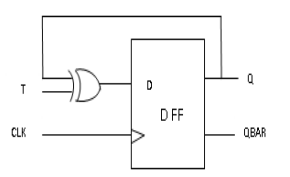
\includegraphics[width=0.5\textwidth]{images/fig1_tff_block.png}
	\caption{T Flip-Flop}
	\label{fig:tff}
\end{figure}

\section{Architecture of Proposed Flip-Flop}

The proposed flip-flop architecture integrates sleepy stack inverters, employing a leakage power reduction technique vital in sub-0.1~$\mu$m feature-size technologies. Replacing static CMOS inverters in the conventional DDFF, this adaptation is prompted by the escalating leakage power observed as feature sizes diminish. Utilizing low threshold voltage transistors in such technology brings the risk of heightened leakage due to reduced supply voltages and threshold voltages.

The sleepy stack technique, combining sleep and forced-stack methods, relies on high-threshold-voltage transistors and a stacked effect to curtail leakage power effectively. Fig.~\ref{fig:ssi} illustrates the sleepy stack inverter's configuration, featuring high-threshold-voltage transistors (P1, P2, N1, N2), along with low-threshold-voltage transistors (P3, N3). Notably, P2 and N2 function as sleep transistors operating in two modes: Active and Sleep.

\subsection{Active Mode}

During the active mode of the sleepy stack inverter ($S=0$, $\bar{S}=1$), the pivotal sleep transistors, P2 and N2, remain consistently activated. This continuous state of activation is fundamental to the inverter's swift and efficient functionality. The persistent engagement of sleep transistors facilitates rapid switching times, enabling seamless logic propagation within the circuit.

In this mode, the sleep transistors, serving as gatekeepers, maintain an open state, enabling a direct flow of logic values from source to drain. This consistent path, established by the activated sleep transistors, ensures a swift and unhindered transfer of logic values across the circuitry. Importantly, this direct path operates independently of the statuses of the transistors parallel to the sleep transistors (P1, P3, N1, N3).

The active mode's strategic utilization of sleep transistors in an ``always-on'' state allows for a streamlined flow of logic signals, optimizing the functionality and efficiency of the sleepy stack inverter. By facilitating faster switching times and preserving a direct logic path, this mode plays a crucial role in reducing propagation delays and enhancing the overall performance of the circuit, especially in scenarios demanding rapid signal processing.

\subsection{Sleep Mode}

During the sleep mode of the sleepy stack inverter ($S=1$, $\bar{S}=0$), a pivotal transition occurs as the sleep transistors P2 and N2 are intentionally switched OFF. However, the effective maintenance of exact logic states within the design is ensured by the transistors running parallel to the sleep transistors, despite their disengagement. This strategic configuration aims to curtail leakage power by employing two distinctive methodologies.

First, the incorporation of high-threshold-voltage transistors aligned in parallel with the sleep transistors acts as a barrier to block any potential leakage current. This configuration effectively mitigates the likelihood of leakage, strategically utilizing the inherent attributes of high-$V_{th}$ transistors to prevent unnecessary current flow.

Second, the exploitation of the stack effect, a phenomenon derived from the coordinated operation of transistors, notably contributes to leakage reduction. By organizing the transistors in a stacked arrangement (P1, P3, N1, N3), a stack effect is harnessed. This effect capitalizes on the simultaneous deactivation of stacked transistors, leading to a substantial reduction in leakage current. For instance, when the logic state $A=1$, the stacked NMOS transistors (N1, N3) are switched ON, while the stacked PMOS transistors (P1, P3) are turned OFF. This coordinated deactivation of stacked PMOS transistors effectively prevents any leakage current passage.

However, while this configuration significantly reduces leakage power, it necessitates a trade-off in terms of the circuit's area footprint. The implementation of multiple transistors and their strategic arrangements, crucial for leakage reduction, inherently impacts the overall area efficiency of the design.

\subsection{Operation of Proposed Flip-Flop}

The schematic representation of the proposed flip-flop harnesses the advantages of the sleepy stack inverter pair, emphasizing significant reductions in overall leakage power and total power consumption. This innovative flip-flop configuration, functioning akin to the conventional DDFF, seamlessly executes the critical evaluation and pre-charge phases.

During the evaluation phase, pivotal input latching takes place, while the subsequent pre-charge phase ensures the steadfast retention of output values. Operating with an overlapping period ($T_{ov}$) of 61~ps and a supply voltage of 1.8~V, this flip-flop design demonstrates impressive operational characteristics. The observed hold times for logic~0 ($T_{ho}$) and logic~1 ($T_{ht}$) stand at 24~ps and 35~ps, respectively.

Mitigating the risk of the race-around problem, the synchronous operation ensured by the 1--1 overlap of CLK and CLK-B guarantees stability within the flip-flop architecture.

Moreover, the versatility of the proposed D flip-flop utilizing the sleepy stack inverter pair extends beyond its primary function, allowing for the derivation of a T flip-flop variant (as depicted in Fig.~\ref{fig:tff}). This derived T flip-flop exhibits a noticeable reduction in power consumption compared to its conventional counterpart, signifying the efficiency gains inherent in the proposed design methodology.

\subsection{Proposed D Flip-Flop with Sleepy Stack Inverter Pair}

The flip-flop design depicted in Fig.~\ref{fig:proposed_dff} incorporates a pair of sleepy stack inverters, presenting an opportunity for comprehensive power reduction during the flip-flop's sleep mode while maintaining functionality akin to a conventional D flip-flop (DDFF) in its evaluation and pre-charge phases.

\begin{figure}[!ht]
	\centering
	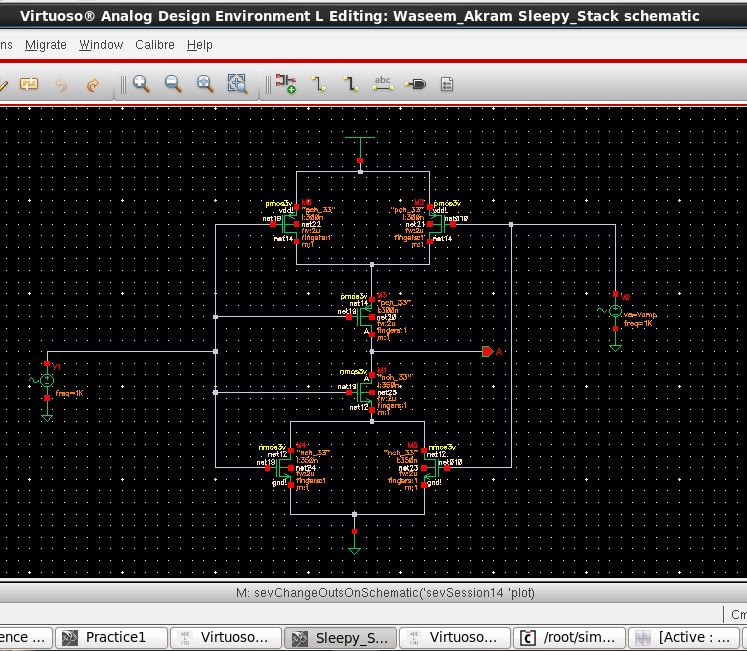
\includegraphics[width=0.5\textwidth]{images/fig2_ssi_schematic.png}
	\caption{Sleepy Stack Inverter Circuit}
	\label{fig:ssi}
\end{figure}

\begin{figure}[!ht]
	\centering
	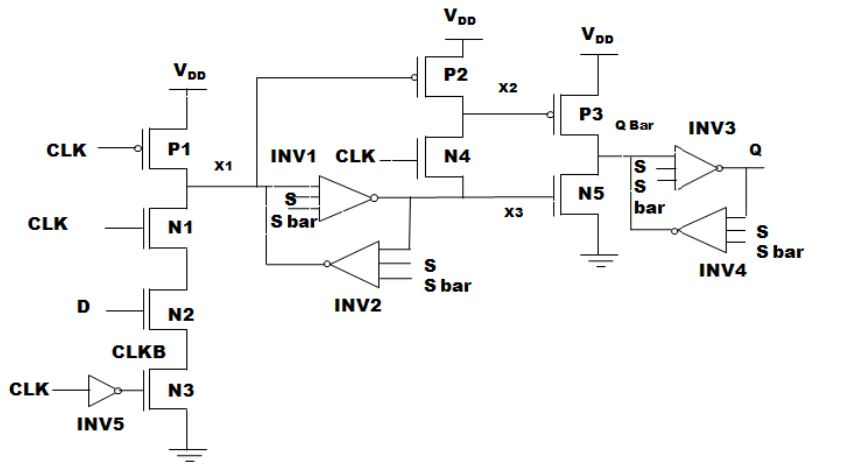
\includegraphics[width=0.5\textwidth]{images/fig3_proposed_dff.png}
	\caption{Proposed D Flip-Flop}
	\label{fig:proposed_dff}
\end{figure}

\begin{figure}[!ht]
	\centering
	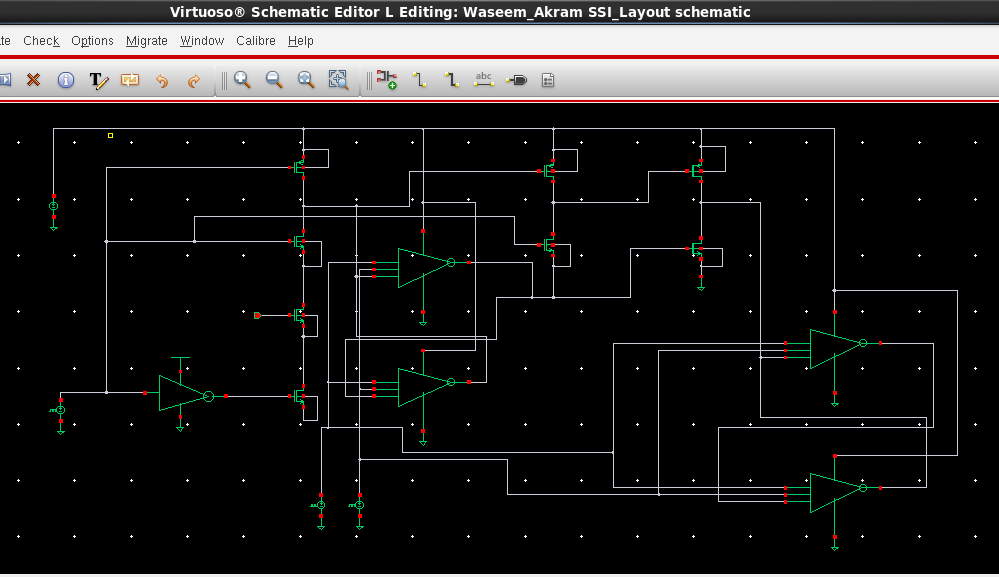
\includegraphics[width=0.5\textwidth]{images/fig4_dff_ssi_circuit.png}
	\caption{DFF-SSI Circuit}
	\label{fig:dff_ssi}
\end{figure}

\section{Results}

\subsection{Operational Phases and Timing Characteristics}

Operational phases involve the evaluation stage, where the flip-flop securely latches the input signal, ensuring the circuit's proper operation, followed by the pre-charge phase, where the output signal is held for stable data retention. The flip-flop exhibits an optimized 61~ps overlapping period, enhancing operational efficiency. Hold times for logic~0 and logic~1 are respectively noted at 24~ps and 35~ps, guaranteeing data stability within the circuit.

\begin{figure}[!ht]
	\centering
	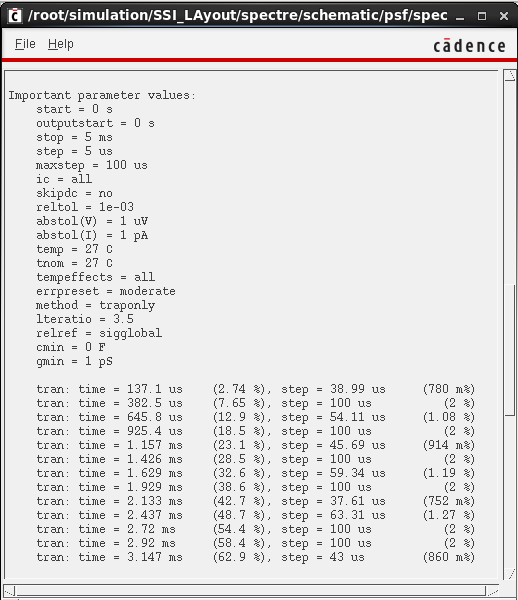
\includegraphics[width=0.4\textwidth]{images/fig5_sim_log_1.png}
	\caption{Spectre transient simulation log (part 1)}
	\label{fig:sim1}
\end{figure}

\begin{figure}[!ht]
	\centering
	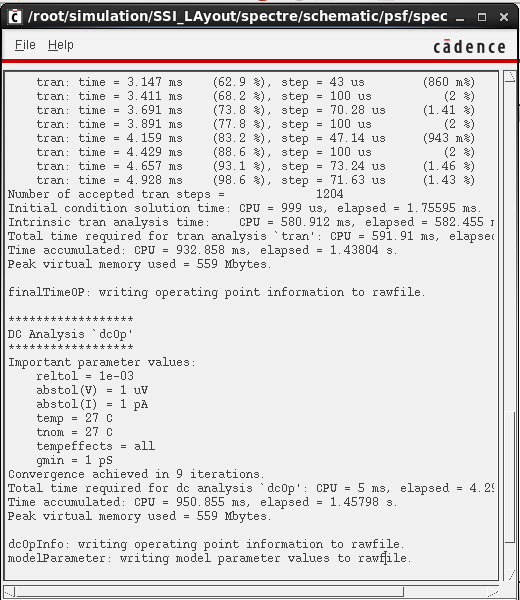
\includegraphics[width=0.4\textwidth]{images/fig6_sim_log_2.png}
	\caption{Spectre DC operating-point simulation log}
	\label{fig:sim2}
\end{figure}

\subsection{Mitigating Race-Around Issues}

Overcoming the race-around issue is achieved through the utilization of a 1--1 overlap strategy between CLK and CLKB signals, ensuring the mitigation of potential timing hazards or data inconsistency.

\subsection{Extension to T Flip-Flops and Efficiency Showcase}

The proposed D flip-flop design utilizing sleepy stack inverters serves as a foundation for T flip-flop designs (Fig.~\ref{fig:tff}), showcasing reduced power consumption compared to traditional D and T flip-flop architectures, and highlighting its efficiency across diverse flip-flop configurations.

\subsection{Waveforms}
The transient simulation results confirm the functional correctness of the proposed designs. Fig. 7 illustrates the input and output waveforms of the sleepy stack inverter, demonstrating full logic swing and correct switching behavior. Figures 8 and 9 present the transient responses of the conventional DFF and the proposed DFF-SSI, respectively. The waveforms verify that the proposed design successfully executes the evaluation and pre-charge phases, accurately capturing the input data at the active clock edge without any logic degradation. Furthermore, the proposed DFF-SSI maintains timing characteristics identical to the conventional baseline, confirming that the integration of the sleepy stack inverters does not introduce functional glitches or timing violations.

\begin{figure}[!ht]
	\centering
	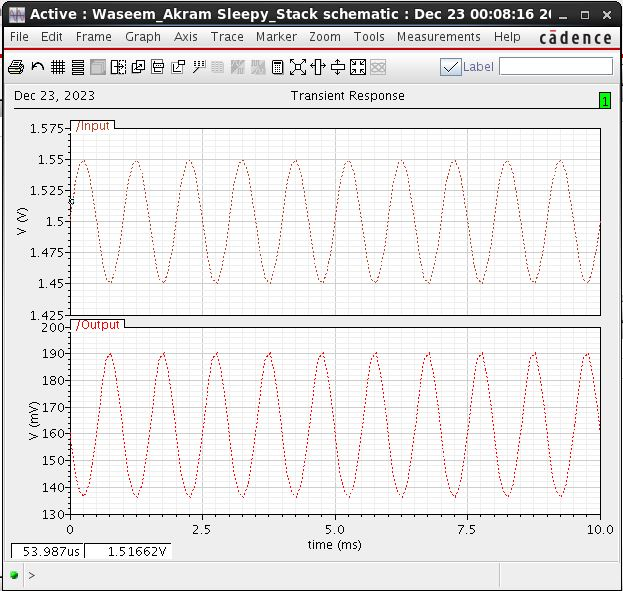
\includegraphics[width=0.5\textwidth]{images/fig7_ssi_waveform.png}
	\caption{Sleepy Stack transient response}
	\label{fig:ssi_graph}
\end{figure}

\begin{figure}[!ht]
	\centering
	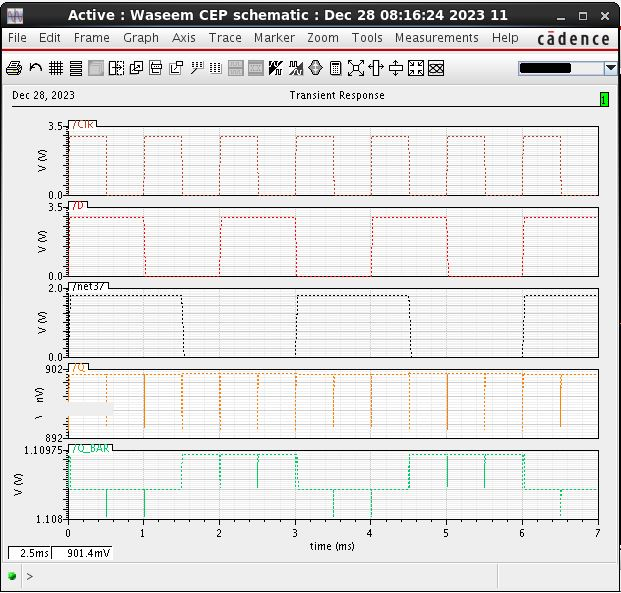
\includegraphics[width=0.5\textwidth]{images/fig8_dff_cmos_waveform.png}
	\caption{Conventional DFF (CMOS) transient response}
	\label{fig:cmos_graph}
\end{figure}

\begin{figure}[!ht]
	\centering
	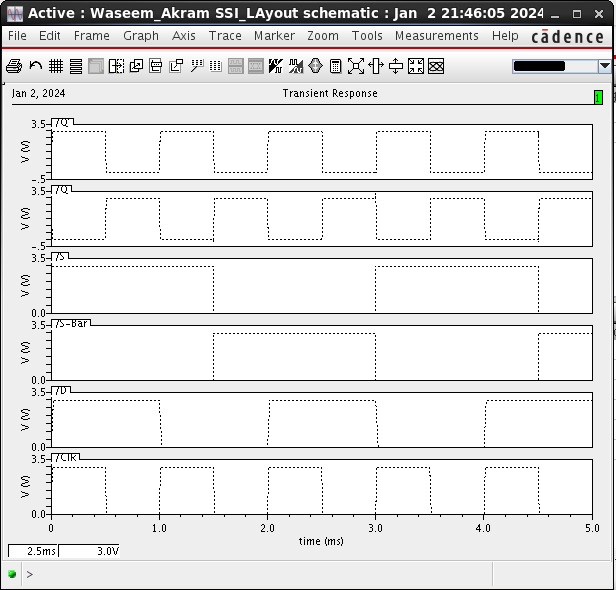
\includegraphics[width=0.5\textwidth]{images/fig9_dff_ssi_waveform.png}
	\caption{Proposed DFF-SSI transient response}
	\label{fig:ssi_results}
\end{figure}

\subsection{Experimental Setup and Simulation Results}

\begin{itemize}
	\item \textbf{Simulation Parameters and Comparative Analysis:} Simulations were conducted using 90nm technology within Cadence Virtuoso, maintaining a consistent supply voltage of 1.8~V for the entire analysis. Comparative studies between static CMOS inverters and sleepy stack inverters revealed a substantial reduction in leakage power by 99\% and a total power reduction of 13.8\% for sleepy stack inverters, as outlined in Table~\ref{tab:inverter}.
	\item \textbf{Flip-Flop Performance Analysis:} Operating the flip-flop at a clock frequency of 1~GHz, with negative setup time and positive hold time concerning the 1--1 overlap of CLK and CLKB, various parameters such as power, delay, and power-delay product (PDP) were computed.
    Comparative analysis of conventional D and T flip-flops versus the proposed variants demonstrated remarkable power reductions, as detailed in Table~\ref{tab:dff}. Total power decreased by 20\% and 15\% respectively, and the leakage power dropped by 89\% and 85\% in the proposed variants. The complete performance breakdowns for the conventional and proposed flip-flops are provided in Table~\ref{tab:conv_ff} and Table~\ref{tab:prop_ff}.
    \item \textbf{Data Activity Impact on Power Consumption:} The examination extended to different data activity levels (25\%, 50\%, 0\%, and 100\%) within the flip-flops, with the total power dissipated shown in Table~\ref{tab:activity}. The results reveal that the proposed designs exhibited lower total power consumption at 25\% and 0\% data activities compared to their conventional counterparts.
    However, at 100\% data activity, both conventional and proposed flip-flops consumed an approximately equal amount of power. It was noted that the switching power dissipation led to the highest total power observed in the T flip-flop configuration.
	\item \textbf{Static Leakage Analysis:} Further analysis explored the static leakage performance of flip-flops across various input and output patterns. Notably, when CLK~=~1 and D~=~0, resulting in Q~=~0, the static leakage was minimized. This observation highlights the dependence of run-time leakage power and total power on input vectors, concluding that different input--output patterns significantly influence the flip-flops' static leakage performance.
\end{itemize}

\begin{table}[H]
	\centering
	\caption{Performance of Inverter}
	\label{tab:inverter}
	\begin{tabular}{lcc}
		\hline
		Inverter Type & Leakage Power (pW) & Total Power (nW) \\
		\hline
		CMOS         & 4041.1  & 414   \\
		Sleepy Stack & 3.2508  & 356.8 \\
		\hline
	\end{tabular}
\end{table}

\begin{table}[H]
	\centering
	\caption{Performance of D Flip-Flop}
	\label{tab:dff}
	\begin{tabular}{lcccc}
		\hline
		Flip-Flop Type & Leakage Power (nW) & Total Power ($\mu$W) & Delay (ns) & PDP (fJ) \\
		\hline
		Conventional & 52.596 & 63.25 & 4.6205 & 292.25 \\
		Proposed     & 5.7438 & 50.44 & 4.6175 & 232.91 \\
		\hline
	\end{tabular}
\end{table}

\begin{table}[H]
	\centering
	\caption{Total Power Dissipated at Different Data Activities by D Flip-Flop}
	\label{tab:activity}
	\begin{tabular}{lcccc}
		\hline
		& \multicolumn{4}{c}{Switching Activity (Total Power, $\mu$W)} \\
		\cline{2-5}
		Flip-Flop Type & 100\% & 50\% & 25\% & 0\% \\
		\hline
		Conventional & 76.96 & 73.20 & 63.17 & 14.35 \\
		Proposed     & 76.67 & 82.68 & 58.97 & 13.65 \\
		\hline
	\end{tabular}
\end{table}

\begin{table}[H]
	\centering
	\caption{Performance of Conventional Flip-Flops}
	\label{tab:conv_ff}
	\begin{tabular}{lcccc}
		\hline
		Conventional Flip-Flop & Leakage Power (nW) & Total Power ($\mu$W) & Delay (ns) & PDP (fJ) \\
		\hline
		D Flip-Flop & 52.596 & 63.25 & 4.6205 & 292.25 \\
		T Flip-Flop & 55.404 & 93.55 & 2.6100 & 244.17 \\
		\hline
	\end{tabular}
\end{table}

\begin{table}[H]
	\centering
	\caption{Performance of Proposed Flip-Flops}
	\label{tab:prop_ff}
	\begin{tabular}{lcccc}
		\hline
		Proposed Flip-Flop & Leakage Power (nW) & Total Power ($\mu$W) & Delay (ns) & PDP (fJ) \\
		\hline
		D Flip-Flop & 5.7438 & 50.44 & 4.6175 & 232.91 \\
		T Flip-Flop & 8.0514 & 78.90 & 2.6065 & 205.65 \\
		\hline
	\end{tabular}
\end{table}

\section{Conclusion}

This paper presented a low-power hybrid flip-flop design that integrates sleepy stack inverters into the static stage of a conventional DDFF. Implemented in Cadence Virtuoso 90nm and simulated at 1~GHz with a 1.8~V supply, the proposed design achieved a 20\% reduction in total power and an 89\% reduction in leakage power compared to the conventional DDFF baseline, with a negligible delay penalty. A derived T flip-flop variant demonstrated 85\% leakage reduction and 15\% total power reduction. Data-activity analysis showed the design's advantage is most pronounced at low switching activity, where leakage dominates. The sleepy stack technique thus offers a promising path toward energy-efficient sequential logic in advanced technology nodes, at the cost of a modest area overhead.

\begin{thebibliography}{00}

\bibitem{b1} J.~C. Park and V.~J. Mooney III, ``Sleepy stack leakage reduction,'' \textit{IEEE Trans. Very Large Scale Integr. (VLSI) Syst.}, vol.~14, no.~11, pp. 1250--1263, Nov. 2006.

\bibitem{b2} K. Absel, L. Manuel, and R.~K. Kavitha, ``Low-power dual dynamic node pulsed hybrid flip-flop featuring efficient embedded logic,'' \textit{IEEE Trans. Very Large Scale Integr. (VLSI) Syst.}, vol.~21, no.~9, pp. 1693--1704, Sep. 2013.

\bibitem{b3} O. Sarbishei and M. Maymandi-Nejad, ``Power-delay efficient overlap-based charge-sharing free pseudo-dynamic D flip-flops,'' in \textit{Proc. IEEE Int. Symp. Circuits Syst.}, May 2007, pp. 637--640.

\bibitem{b4} O. Sarbishei and M. Maymandi-Nejad, ``A novel overlap-based logic cell: An efficient implementation of flip-flops with embedded logic,'' \textit{IEEE Trans. Very Large Scale Integr. (VLSI) Syst.}, vol.~18, no.~2, pp. 222--231, Feb. 2010.

\end{thebibliography}
\end{document}